\documentclass{article}

\makeatletter
\def\input@path{{COMP_5970_6970_Course_Project_Template/}}
\makeatother
\usepackage[final]{neurips_2024}
\usepackage[utf8]{inputenc}
\usepackage[T1]{fontenc}
\usepackage{microtype}
\usepackage{url}
\usepackage{booktabs}
\usepackage{amsmath,amssymb,amsfonts}
\usepackage{graphicx}
\usepackage{subcaption}
\usepackage{multirow}
\usepackage{enumitem}
\usepackage{xcolor}
\usepackage{tikz}
\usetikzlibrary{arrows.meta,positioning,fit,calc}
\usepackage{xspace}

\graphicspath{{figs/}}

\definecolor{anchorblue}{RGB}{34,94,168}
\definecolor{quantred}{RGB}{168,72,34}
\definecolor{servergold}{RGB}{184,134,11}
\definecolor{buffergreen}{RGB}{44,122,95}

\newcommand{\method}{AGD-Smart\xspace}
\DeclareMathOperator*{\argmax}{arg\,max}

\title{Anchor-Guided Dequantization for Federated Learning}
\author{
  Jacob Simmons\\
  Auburn University\\
  \texttt{jss0112@auburn.edu}
  \And
  Owen Strength\\
  Auburn University\\
  \texttt{ods0005@auburn.edu}
}

\begin{document}

\maketitle

\begin{abstract}
Federated learning systems often mix clients with very different hardware
budgets. Some clients can transmit full-precision model updates, while others
must aggressively quantize before upload. That mismatch introduces systematic
bias into server aggregation. We study a server-side correction approach,
\method, that uses full-precision \emph{anchor} clients to supervise a residual
CorrectionNet for low-bit client deltas. The implementation combines
client-to-anchor smart matching, a replay buffer over recent rounds, optional
distillation on a server validation split, warmup before correction is applied,
and direction-preserving blending at inference time. Across the reported
configurations, \method consistently outperforms the simplified ProWD baseline
by 1.9--5.7 percentage points. Its strongest gains appear under severe INT2
quantization, where it outperforms FedAvg by +14.2 points at round 10 and
remains ahead by +2.1 points at round 50.
\end{abstract}

\section{Introduction}

Federated learning (FL) trains a shared model across many clients without
centralizing raw data \citep{mcmahan2017}. In practice, however, participating
devices are rarely homogeneous. A laptop-class client may upload a
full-precision update, while an embedded device or phone may need INT8, INT4,
or even INT2 quantization to fit its communication and memory budget. Once
those updates are averaged together, quantization error no longer behaves like
benign noise; it becomes a structured bias in the aggregated direction.

This project studies a simple question: can a server learn to reverse some of
that bias if a small subset of clients still provide clean, full-precision
updates? We use those full-precision clients as \emph{anchors}. Their updates
provide round-level supervision for a server-side CorrectionNet that maps a
quantized delta toward a more full-precision-like delta before aggregation.

That question sits at the intersection of two existing FL lines of work.
Heterogeneity-aware optimizers such as FedProx, SCAFFOLD, and FedNova study how
client drift and uneven local progress affect aggregation
\citep{li2020fedprox,karimireddy2020scaffold,wang2020fednova}. Mixed-precision
and bit-width-aware methods such as ProWD, FedShift, and recent client-specific
quantization schemes instead focus on what happens when clients cannot all
communicate at the same precision
\citep{yoon2022prowd,seo2024fedshift,chen2024fedmpq}.

The current implementation goes beyond a naive dequantizer in several ways.
Instead of training on only the current round, it keeps a replay buffer over the
most recent rounds. Instead of forcing every low-bit client toward the same
anchor mean, it can assign each constrained client its most similar anchor by
cosine similarity. It also supports an optional distillation term computed on a
server validation set and blends corrected deltas with the original quantized
delta to preserve client-specific direction under non-IID data.

Our main contributions are:
\begin{itemize}[leftmargin=*]
  \item A template-based writeup of the implemented anchor-guided correction
  pipeline, including warmup, replay buffering, smart matching, normalization,
  and optional similarity-aware aggregation.
  \item A reusable architecture diagram that makes the per-round data flow and
  supervision path explicit.
  \item An empirical summary showing that the method is most useful in the
  severe quantization regime, especially INT2, while still improving over the
  simplified ProWD baseline in every reported configuration and matching or
  beating FedShift on the shared settings, with the clearest gains at early
  INT2, final INT4, and non-IID INT8.
\end{itemize}

\section{Related Work}

FedAvg remains the standard FL baseline because of its simplicity and strong
performance when client updates are already directionally compatible
\citep{mcmahan2017}. Later optimization work made the heterogeneity problem more
explicit. FedProx adds proximal regularization to stabilize training when local
objectives and available local work differ across clients \citep{li2020fedprox}.
SCAFFOLD corrects client drift with control variates
\citep{karimireddy2020scaffold}, while FedNova analyzes objective inconsistency
under unequal local progress and fixes it through normalized aggregation
\citep{wang2020fednova}. These methods are important context because they show
that even before quantization, federated aggregation is already sensitive to
client mismatch.

Communication-efficient learning introduces another axis: compression. QSGD is
an influential quantized optimization method in distributed training
\citep{alistarh2017qsgd}, and FedPAQ brings periodic averaging plus quantized
message passing into the FL setting \citep{reisizadeh2020fedpaq}. More recent
work pushes this further toward resource-aware mixed precision. For example,
Chen and Vikalo propose client-specific mixed-precision quantization for
resource-constrained heterogeneous devices \citep{chen2024fedmpq}. Those papers
primarily study how to train and communicate efficiently under low precision,
whereas this project focuses on repairing the low-bit uploads after they arrive
at the server.

The closest prior work is ProWD, which explicitly targets bit-width
heterogeneous FL through a server-side dequantizer
\citep{yoon2022prowd}. FedShift addresses the same mixed-precision aggregation
problem from a different angle by using weight shifting to align client updates
before aggregation \citep{seo2024fedshift}. Our implementation sits in this
same mixed-precision corridor, but it differs in three practical ways: it uses
full-precision anchor clients as direct supervision, it trains the corrector on
a replayed history instead of only the current round, and it uses smart
client-to-anchor matching rather than a single global target. The result should
therefore be read as a server-side, anchor-supervised dequantization variant
positioned between plain FedAvg and recent mixed-precision correction methods.

\section{Method}

\subsection{Setting}

At each communication round, the server broadcasts the current global model to
all clients. Anchor clients return full-precision updates, while constrained
clients return low-bit quantized updates. The server's job is to repair the
constrained uploads before aggregation without disturbing the clean anchor
signal.

\begin{figure*}[t]
  \centering
  {\def\methoddiagramfont{\normalsize}%
  \resizebox{0.99\textwidth}{!}{\providecommand{\methoddiagramfont}{\small}

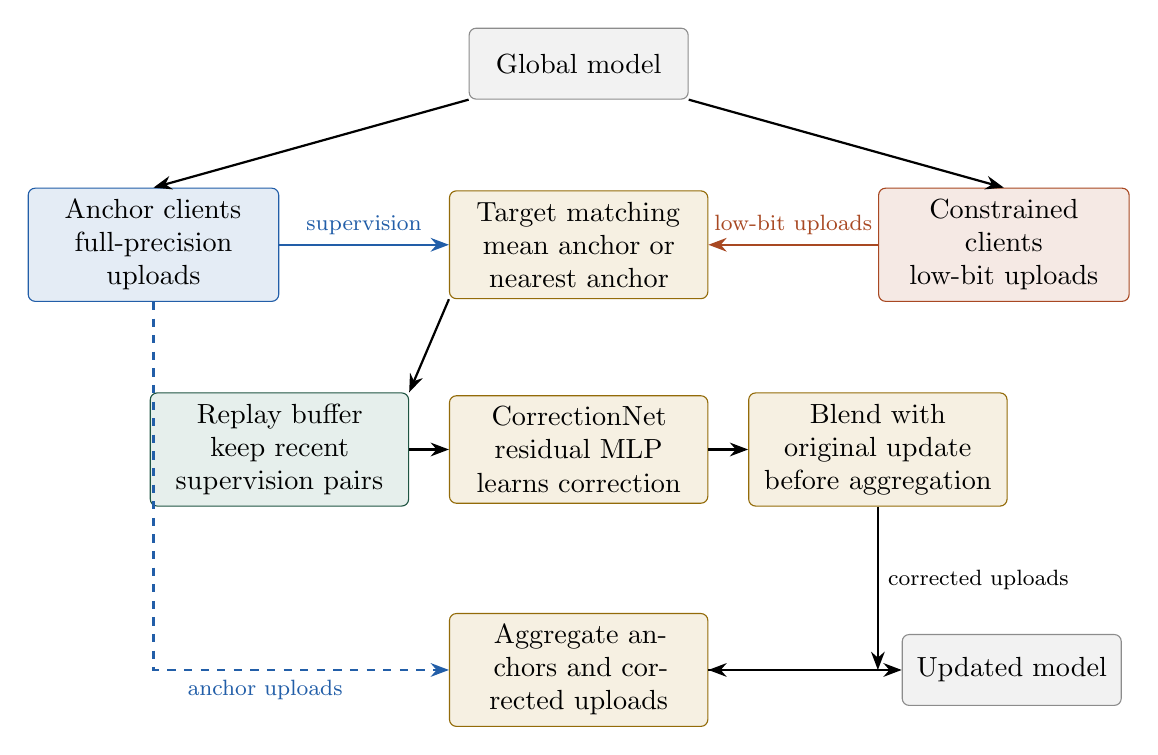
\begin{tikzpicture}[
  >=Stealth,
  font=\methoddiagramfont,
  box/.style={
    draw,
    rounded corners=2.5pt,
    align=center,
    inner sep=4pt,
    minimum height=9mm
  },
  model/.style={box, fill=black!5, draw=black!45, text width=2.5cm},
  anchorbox/.style={box, fill=anchorblue!12, draw=anchorblue, text width=2.9cm},
  quantbox/.style={box, fill=quantred!12, draw=quantred, text width=2.9cm},
  serverbox/.style={box, fill=servergold!12, draw=servergold!80!black, text width=3.0cm},
  bufferbox/.style={box, fill=buffergreen!12, draw=buffergreen!70!black, text width=3.0cm}
]

\node[model] (global) at (0, 0) {Global model};

\node[anchorbox] (anchors) at (-5.4, -2.3) {Anchor clients\\full-precision uploads};
\node[serverbox] (targets) at (0, -2.3) {Target matching\\mean anchor or nearest anchor};
\node[quantbox] (quantized) at (5.4, -2.3) {Constrained clients\\low-bit uploads};

\node[bufferbox] (replay) at (-3.8, -4.9) {Replay buffer\\keep recent supervision pairs};
\node[serverbox] (corrnet) at (0, -4.9) {CorrectionNet\\residual MLP learns correction};
\node[serverbox] (blend) at (3.8, -4.9) {Blend with original update\\before aggregation};

\node[serverbox] (agg) at (0, -7.7) {Aggregate anchors and corrected uploads};
\node[model] (next) at (5.5, -7.7) {Updated model};

\coordinate (aggleft) at ([xshift=-0.8cm]agg.west);
\coordinate (aggright) at ([xshift=0.8cm]agg.east);
\coordinate (blenddrop) at (blend.south |- aggright);

\draw[->, thick] (global.south west) -- (anchors.north);
\draw[->, thick] (global.south east) -- (quantized.north);
\draw[->, thick, anchorblue] (anchors.east) -- node[above, font=\footnotesize] {supervision} (targets.west);
\draw[->, thick, quantred] (quantized.west) -- node[above, font=\footnotesize] {low-bit uploads} (targets.east);
\draw[->, thick] (targets.south west) -- (replay.north east);
\draw[->, thick] (replay.east) -- (corrnet.west);
\draw[->, thick] (corrnet.east) -- (blend.west);
\draw[->, thick] (blend.south) -- node[pos=0.45, right, font=\footnotesize] {corrected uploads} (blenddrop);
\draw[->, thick] (blenddrop) -- (aggright) -- (agg.east);
\draw[->, thick, anchorblue, dashed] (anchors.south) |- node[pos=0.74, below, font=\footnotesize] {anchor uploads} (aggleft) -- (agg.west);
\draw[->, thick] (agg.east) -- (next.west);

\end{tikzpicture}
}}
  \caption{Implemented round-level pipeline for anchor-guided dequantization.
  Full-precision anchor clients supervise a server-side correction model. The
  server matches constrained uploads to anchor targets, reuses recent
  supervision through a replay buffer, applies a learned correction, blends it
  with the original low-bit update, and aggregates the repaired uploads with
  the anchors.}
  \label{fig:method_architecture}
\end{figure*}

\subsection{Target Construction}

The correction module operates only on \emph{learnable} parameters. BatchNorm
running statistics bypass the correction path unchanged. Each client delta is
flattened into a single vector before training the corrector.

Two target modes are implemented. In the simpler version, every constrained
client is trained toward the mean anchor update for that round. In the smart
matching version, each constrained client is paired with the anchor whose update
has the highest cosine similarity. The smart-matching version is the one
reported as \method.

\subsection{Correction Network and Replay Buffer}

The server trains a residual MLP, CorrectionNet, on pairs of quantized uploads
and anchor-derived targets. The network uses one encoder layer, three residual
blocks, and a zero-initialized decoder so that it starts close to the identity
map and only has to learn a correction rather than a full replacement update.

Instead of training only on the current round, the server appends each new
mini-batch of supervision pairs to a replay buffer capped at the most recent 10
rounds. All buffered pairs are concatenated for training. Before the correction
update, buffered quantized deltas are normalized with a single scalar
$z$-score computed across the buffer so that the network sees a more stable
input scale from round to round.

\subsection{Training Objective}

The base training signal is a reconstruction loss that pushes corrected uploads
toward their anchor-derived targets. When a server validation loader is
available, the implementation can also add a distillation term. In that case,
the current global model acts as the teacher, and the corrected update is also
encouraged to produce similar logits on the validation split.

The teacher logits come from the current global model on the validation split.
The student logits come from a model built by applying the mean corrected delta
from the current round. The reported configurations use distillation
temperature $\tau=4$.

\subsection{Applying Correction and Aggregation}

At inference time, the server denormalizes the network output and can blend the
corrected upload with the original quantized upload. The main smart-matching
configuration uses an 80/20 mix of corrected and original update, which helps
preserve client-specific direction under non-IID data.

The corrected deltas are then aggregated together with anchor deltas. The code
supports either plain sample-count weighting or a convex combination of
sample-count and cosine-similarity weights relative to the mean anchor delta.
Finally, the aggregated update is applied to the global model.

\subsection{Warmup}

The smart-matching strategy also uses a warmup phase. For the first five rounds,
the server trains the CorrectionNet and fills the replay buffer but still
aggregates the raw client deltas with FedAvg. Correction is only applied after
the buffer contains enough supervision signal to avoid harming early
optimization.

\section{Experimental Setup}

\textbf{Dataset and partitioning.}
All reported experiments use CIFAR-10. Near-IID settings use a large Dirichlet
concentration ($\alpha=100$), while the heterogeneous setting uses
$\alpha=0.5$.

\textbf{Model and local training.}
Clients train a shared CNN for two local epochs per communication round. The
server-side CorrectionNet uses hidden width 256.

\textbf{Client types.}
Each experiment uses 10 total clients with full participation. Anchor fractions
range from 20\% to 50\%, depending on the configuration.

\textbf{Baselines.}
We compare against FedAvg \citep{mcmahan2017} and a simplified ProWD-style
baseline derived from \citet{yoon2022prowd}. The simplified ProWD baseline
implemented in this repository uses a shared three-layer residual MLP trained
only on the current round and targets the mean anchor delta.

\textbf{Reported configurations.}
Table~\ref{tab:configs} summarizes the main settings referenced in the paper and
slides.

\begin{table}[h]
  \centering
  \caption{Reported experimental configurations.}
  \label{tab:configs}
  \small
  \resizebox{0.95\columnwidth}{!}{%
  \begin{tabular}{lccccc}
    \toprule
    Setting & $\alpha$ & Bits & Anchors & Rounds & Corr. epochs \\
    \midrule
    Near-IID ProWD benchmark & 100 & INT8 & 5 / 10 & 50 & 5 \\
    Near-IID severe quant.   & 100 & INT2 & 2 / 10 & 50 & 20 \\
    Near-IID moderate quant. & 100 & INT4 & 5 / 10 & 50 & 10 \\
    Non-IID heterogeneous    & 0.5 & INT8 & 5 / 10 & 50 & 5 \\
    \bottomrule
  \end{tabular}}
\end{table}

This table is mainly an interpretation guide for the later accuracy results.
The near-IID INT8 row is the easiest setting and is closest to the regime where
plain averaging is already strong. The INT2 row is much harsher: only two
anchors supervise eight constrained clients, and each coordinate is compressed
to just three effective levels. Because the rows differ in both bit-width and
anchor fraction, the most important comparisons are within each row across
methods, while the cross-row trend tells us when correction becomes necessary.

\textbf{Evaluation.}
The primary metric is top-1 accuracy on the global CIFAR-10 test set at
selected communication rounds. We focus on round 10 to measure early usefulness
and round 50 to measure whether gains persist.

\section{Results}

\subsection{Main Result: INT2 Is the Regime Where Correction Matters}

Figure~\ref{fig:int2_curve} shows the strongest result in the project: near-IID
CIFAR-10 with INT2 quantization and only 20\% anchors. This is the regime where
plain averaging struggles most because each uploaded coordinate has only three
effective levels.

\begin{figure}[h]
  \centering
  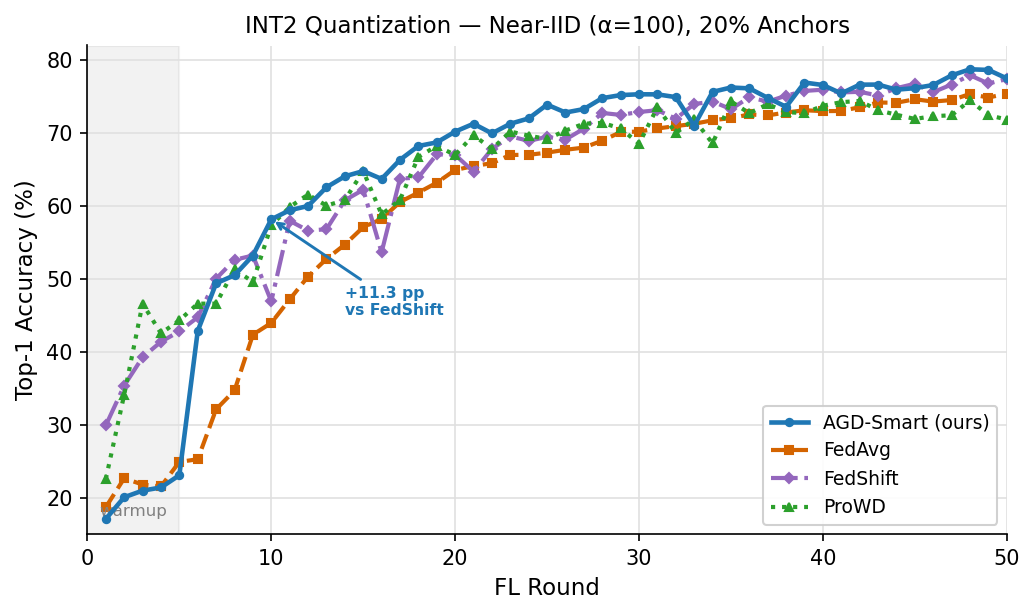
\includegraphics[width=\columnwidth]{int2_curve.png}
  \caption{INT2 near-IID benchmark over 50 rounds. \method gains sharply after
  warmup and stays ahead of FedAvg throughout the full run.}
  \label{fig:int2_curve}
\end{figure}

\begin{table}[h]
  \centering
  \caption{INT2 near-IID checkpoints (\%).}
  \label{tab:int2_checkpoints}
  \begingroup
  \footnotesize
  \setlength{\tabcolsep}{5pt}
  \begin{tabular}{lcccc}
    \toprule
    Method & R10 & R20 & R30 & R50 \\
    \midrule
    FedAvg                    & 44.0 & 64.9 & 70.2 & 75.4 \\
    FedShift                  & 46.9 & 67.0 & 72.9 & 77.4 \\
    ProWD                     & 57.3 & 67.0 & 68.5 & 71.8 \\
    \textbf{\method}          & \textbf{58.2} & \textbf{70.2} & \textbf{75.3} & \textbf{77.5} \\
    \bottomrule
  \end{tabular}
  \endgroup
\end{table}

Table~\ref{tab:int2_checkpoints} shows that \method is the best method at every
reported checkpoint, but the comparison to FedShift changes the interpretation
of the result. FedShift already fixes much of the end-of-training bias: by
round 50 it reaches 77.4, essentially tied with \method at 77.5 and clearly
above FedAvg. The remaining advantage of \method is therefore front-loaded. It
leads FedShift by +11.3 points at round 10 and by +3.2 at round 20, which is
exactly the interval where a communication-limited system benefits most from a
stronger correction policy. Relative to ProWD, the gap still widens over time,
reaching +5.7 at round 50. That separates the three correction strategies
clearly: ProWD forgets too much from round to round, FedShift eventually
recovers but reacts slowly, and \method combines fast activation with strong
final accuracy.

\subsection{Noise Scaling}

Table~\ref{tab:noise_scaling} shows that the method's value is highly dependent
on quantization severity. Once the bit-width rises to INT3 or above, FedAvg is
usually good enough. The correction pipeline becomes most valuable when the
quantized representation collapses too much directional information. FedShift
was rerun only on the four shared headline configurations, so this table keeps
the broader bit-width threshold comparison against FedAvg and ProWD.

\begin{table}[h]
  \centering
  \caption{Round-20 accuracy under different near-IID bit-widths with 20\%
  anchors.}
  \label{tab:noise_scaling}
  \small
  \resizebox{0.95\columnwidth}{!}{%
  \begin{tabular}{lccccc}
    \toprule
    Bits & Levels & FedAvg & ProWD & \method & vs. FedAvg \\
    \midrule
    INT8 & 255 & 72.0 & 66.4 & 68.2 & $-3.9$ \\
    INT6 & 63  & 73.0 & 68.3 & 70.7 & $-2.2$ \\
    INT4 & 15  & 74.5 & 65.4 & 72.8 & $-1.7$ \\
    INT3 & 7   & 74.4 & 65.8 & 71.7 & $-2.8$ \\
    INT2 & 3   & 65.4 & 59.8 & \textbf{70.7} & \textbf{+5.3} \\
    \bottomrule
  \end{tabular}}
\end{table}

Table~\ref{tab:noise_scaling} makes the crossover point very clear. Compared
with ProWD, \method wins at every bit-width, from +1.8 points at INT8 up to
+10.9 points at INT2, so the improved correction design is consistently better
than the simpler learned baseline. Compared with FedAvg, however, the sign of
the gain flips with quantization severity: \method is still 1.7--3.9 points
behind from INT8 through INT3, then jumps to a +5.3 advantage at INT2. That
pattern supports the main claim of the paper. Learned dequantization is not
universally necessary, but it becomes valuable once the quantizer is coarse
enough that plain averaging cannot preserve update direction. The shared
FedShift reruns follow the same story: it is competitive in the easier near-IID
settings and helpful at INT2, but the learned model becomes more valuable once
early convergence or heterogeneous matching matters.

\subsection{Behavior in Milder Regimes}

Figure~\ref{fig:other_curves} summarizes the remaining reported settings. The
pattern is consistent: \method reliably beats ProWD, but it only surpasses
FedAvg once quantization is severe enough that averaging alone can no longer
recover the signal.

\begin{figure*}[t]
  \centering
  \begin{subfigure}{0.32\textwidth}
    \centering
    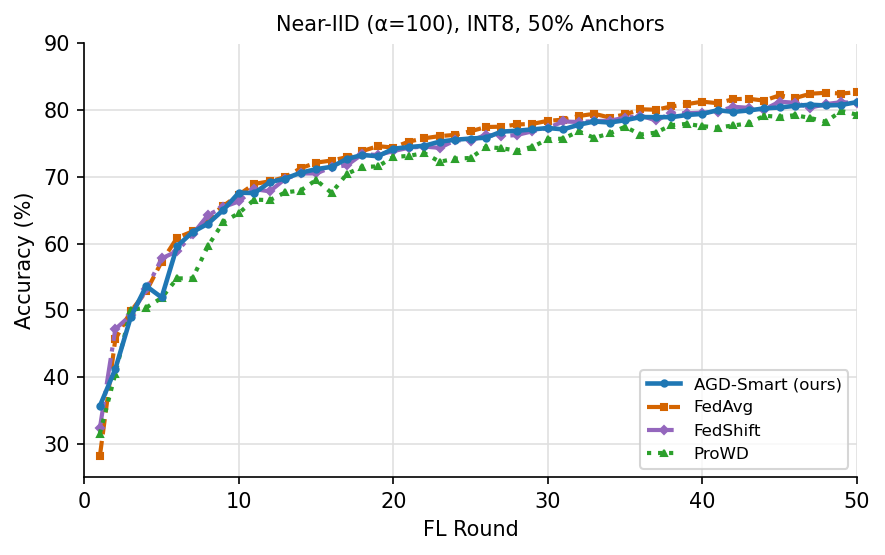
\includegraphics[width=\linewidth]{int8_curve.png}
    \caption{Near-IID, INT8}
  \end{subfigure}\hfill
  \begin{subfigure}{0.32\textwidth}
    \centering
    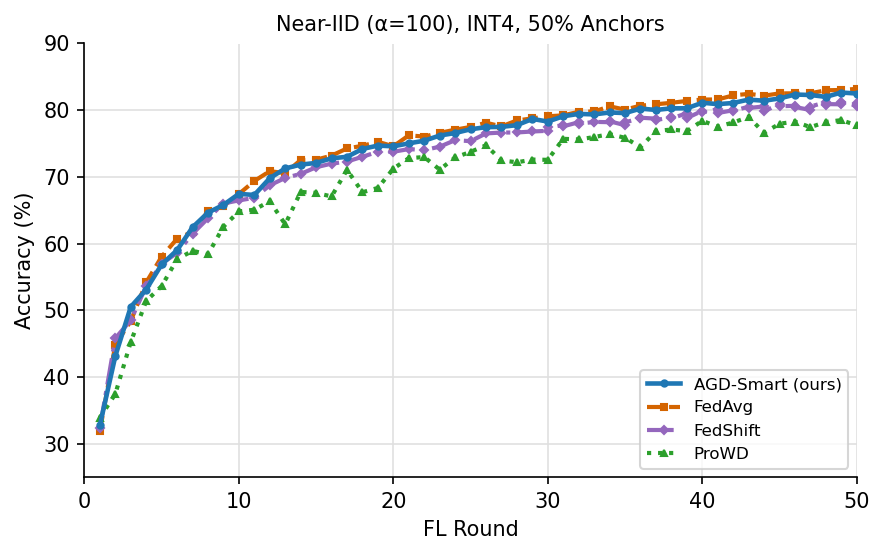
\includegraphics[width=\linewidth]{int4_curve.png}
    \caption{Near-IID, INT4}
  \end{subfigure}\hfill
  \begin{subfigure}{0.32\textwidth}
    \centering
    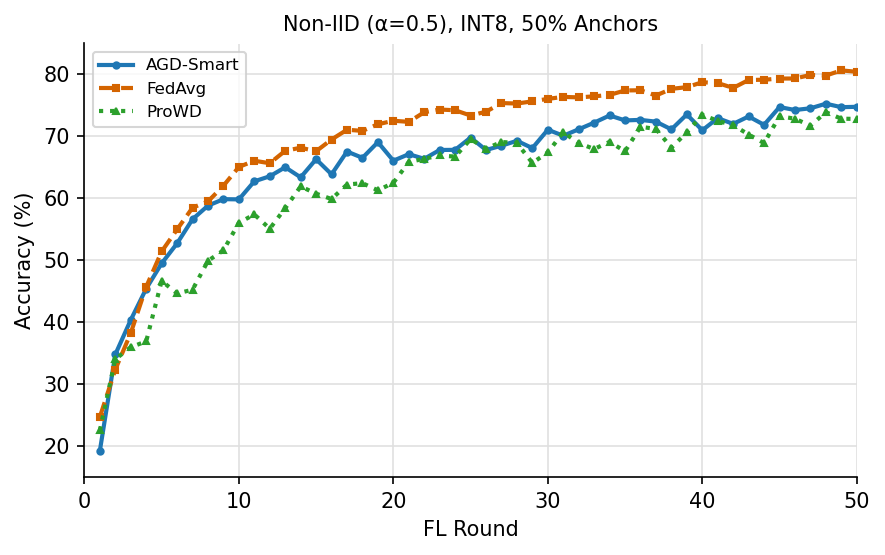
\includegraphics[width=\linewidth]{noniid_curve.png}
    \caption{Non-IID, INT8}
  \end{subfigure}
  \caption{Secondary regimes. The method stays consistently above ProWD, nearly
  matches FedAvg under near-IID INT4, and narrows the gap to FedAvg under
  non-IID INT8 without fully closing it.}
  \label{fig:other_curves}
\end{figure*}

\begin{table*}[t]
  \centering
  \caption{Summary across shared configurations, including FedShift.}
  \label{tab:summary}
  \small
  \resizebox{0.95\textwidth}{!}{%
  \begin{tabular}{lccccc}
    \toprule
    Setting & FedShift @ R50 & \method @ R50 & vs. FedShift & vs. ProWD & vs. FedAvg \\
    \midrule
    Near-IID, INT2, 20\% anchors & 77.4 & 77.5 & +0.1 & +5.7 & +2.1 \\
    Near-IID, INT8, 50\% anchors & 81.1 & 81.2 & +0.1 & +1.9 & -1.5 \\
    Near-IID, INT4, 50\% anchors & 80.7 & 82.5 & +1.8 & +4.8 & -0.7 \\
    Non-IID, INT8, 50\% anchors  & 73.8 & 74.8 & +1.0 & +2.0 & -5.6 \\
    \bottomrule
  \end{tabular}}
\end{table*}

Table~\ref{tab:summary} sharpens the baseline story. FedShift is the stronger
lightweight comparator: it beats ProWD in three of the four shared settings and
nearly matches \method at the easier near-IID endpoints. That makes the INT4
and non-IID rows more informative than the near-IID INT8 tie. At INT4,
\method keeps a +1.8 final advantage over FedShift while finishing within 0.7
of FedAvg. Under non-IID INT8, the final gap is +1.0 and the midpoint gap is
+3.9 at round 25, which suggests that smart client-to-anchor matching matters
more than a single global shift once anchor and constrained populations no
longer share the same mean direction. INT2 is different again: the final
accuracy is nearly tied, but the route to that endpoint is not.

\begin{figure}[t]
  \centering
  \resizebox{0.98\columnwidth}{!}{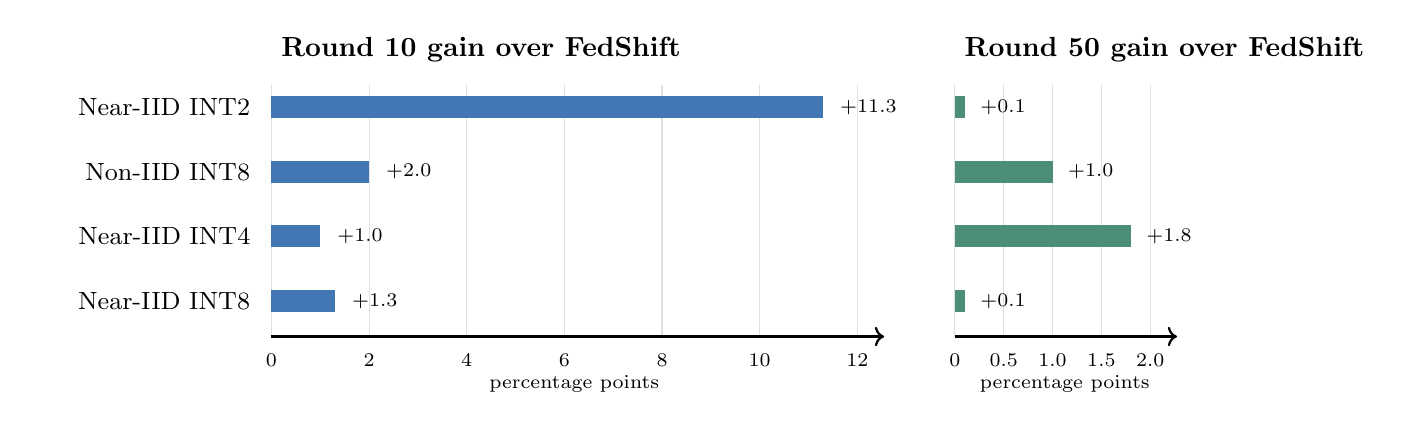
\begin{tikzpicture}[x=0.62cm,y=0.82cm,font=\small]
  \def\barhalf{0.17}

  \node[anchor=west,font=\bfseries] at (0,4.9) {Round 10 gain over FedShift};
  \node[anchor=west,font=\bfseries] at (14,4.9) {Round 50 gain over FedShift};

  \foreach \x/\lab in {0/0,2/2,4/4,6/6,8/8,10/10,12/12} {
    \draw[gray!25] (\x,0.45) -- (\x,4.35);
    \node[font=\scriptsize] at (\x,0.08) {\lab};
  }
  \draw[->,thick] (0,0.45) -- (12.55,0.45);
  \node[font=\scriptsize] at (6.2,-0.28) {percentage points};

  \foreach \x/\lab in {14/0,15/0.5,16/1.0,17/1.5,18/2.0} {
    \draw[gray!25] (\x,0.45) -- (\x,4.35);
    \node[font=\scriptsize] at (\x,0.08) {\lab};
  }
  \draw[->,thick] (14,0.45) -- (18.55,0.45);
  \node[font=\scriptsize] at (16.25,-0.28) {percentage points};

  \foreach \y/\name/\early/\final in {
    4/{Near-IID INT2}/11.3/0.1,
    3/{Non-IID INT8}/2.0/1.0,
    2/{Near-IID INT4}/1.0/1.8,
    1/{Near-IID INT8}/1.3/0.1
  } {
    \node[anchor=east,align=right,text width=2.7cm] at (-0.25,\y) {\name};
    \fill[anchorblue!85] (0,\y-\barhalf) rectangle (\early,\y+\barhalf);
    \node[anchor=west,font=\scriptsize] at (\early+0.15,\y) {+\early};
    \pgfmathsetmacro{\finalx}{14 + 2*\final}
    \fill[buffergreen!85] (14,\y-\barhalf) rectangle (\finalx,\y+\barhalf);
    \node[anchor=west,font=\scriptsize] at (\finalx+0.12,\y) {+\final};
  }
\end{tikzpicture}
}
  \caption{\method's gain over FedShift at round 10 and round 50 on the four
  shared configurations. The largest early-round advantage appears under INT2,
  while the largest persistent end-of-training gain appears at INT4.}
  \label{fig:fedshift_gains}
\end{figure}

Figure~\ref{fig:fedshift_gains} makes that contrast explicit. FedShift is
already a very strong no-learning baseline when the client population is
near-IID. At near-IID INT8 and INT2, the final gap is only +0.1. But those
near ties hide where \method helps most. In the severe INT2 regime it opens an
11.3-point lead by round 10, which matters if communication rounds are scarce.
At INT4, it keeps a meaningful +1.8 end-of-training advantage, suggesting that
the replayed learned corrector is still buying something after simple mean
alignment has done its part. Under non-IID data, FedShift loses more clearly
because the anchor mean is no longer a reliable global target.

\section{Conclusion}

Using the provided course template, this paper reframes the project as a
server-side correction pipeline for bit-width-heterogeneous federated learning.
The central result is not that correction universally beats FedAvg. It does not.
Instead, the evidence points to a narrower and more useful claim: anchor-guided
correction is most valuable when quantization is so aggressive that averaging
cannot reliably reconstruct the true direction of the update.

In that regime, especially INT2, \method provides substantial early-round and
end-of-training gains while remaining consistently stronger than the simplified
ProWD baseline in every reported configuration. The reusable method diagram and
the revised slides emphasize the practical mechanics that drive that result:
anchor supervision, replay buffering, smart matching, warmup, and blended
correction.


\bibliographystyle{unsrtnat}
\bibliography{references}

\end{document}
